\documentclass[border=2pt]{standalone}
% Shared TikZ style contract for every schematic figure in this paper.
% Each schematic is a standalone document that \input's this file, so the
% schematics and the matplotlib data figures form one visual system.
%
% Colours are the same Okabe-Ito values as figures/scifig_style.py.

% No font package: the manuscript class sets the body in Computer Modern, so
% the schematics inherit the same family by loading nothing here.
\usepackage{amsmath,amssymb}
\usepackage{tikz}
\usetikzlibrary{arrows.meta,positioning,calc,fit,backgrounds,shapes.geometric,
                shapes.multipart,patterns,decorations.pathreplacing,matrix}

% ---------- Notation shared with the manuscript ----------
% Kept in sync with the definitions in main.tex so that a symbol means the
% same thing in a schematic as it does in the body.
\newcommand{\Cmax}{C_{\max}}
\newcommand{\Zcost}{Z}
\newcommand{\Nb}{\mathcal{N}}

% ---------- Okabe-Ito colour-blind-safe palette ----------
\definecolor{oiblue}{RGB}{0,114,178}
\definecolor{oiorange}{RGB}{230,159,0}
\definecolor{oigreen}{RGB}{0,158,115}
\definecolor{oivermilion}{RGB}{213,94,0}
\definecolor{oipurple}{RGB}{204,121,167}
\definecolor{oisky}{RGB}{86,180,233}
\definecolor{oiyellow}{RGB}{240,228,66}
\definecolor{oigray}{RGB}{110,110,110}

% ---------- Shared node and arrow styles ----------
\tikzset{
  block/.style={draw, rounded corners=2pt, minimum height=6.5mm, minimum width=17mm,
                align=center, font=\footnotesize, fill=oisky!16, line width=0.6pt,
                draw=oiblue!70},
  keyblock/.style={block, fill=oiorange!26, draw=oiorange!85},
  smallblock/.style={block, minimum height=5mm, minimum width=12mm, font=\scriptsize},
  datanode/.style={draw, trapezium, trapezium left angle=70, trapezium right angle=110,
                   align=center, font=\scriptsize, fill=oigreen!14, line width=0.6pt,
                   draw=oigreen!75, inner sep=2pt},
  opnode/.style={draw, circle, inner sep=1pt, minimum size=6mm, font=\scriptsize,
                 fill=oiyellow!45, line width=0.6pt, draw=oigray},
  macnode/.style={draw, rectangle, rounded corners=1pt, minimum size=6mm,
                  font=\scriptsize, fill=oisky!30, line width=0.6pt, draw=oiblue!70},
  modnode/.style={draw, diamond, aspect=1.4, inner sep=1pt, minimum size=6mm,
                  font=\scriptsize, fill=oipurple!28, line width=0.6pt, draw=oipurple!85},
  arrow/.style={-{Stealth[length=2.0mm]}, line width=0.65pt},
  dasharrow/.style={arrow, dashed, draw=oigray},
  thinedge/.style={line width=0.45pt, draw=oigray},
  note/.style={font=\scriptsize, text=oigray, align=center},
  tinynote/.style={font=\tiny, text=oigray, align=center},
  group/.style={draw=oigray, dashed, rounded corners=3pt, inner sep=2.6mm,
                line width=0.5pt},
  grouplabel/.style={font=\scriptsize\itshape, text=oigray},
  whitebg/.style={fill=white, inner sep=1pt},
}

\begin{document}
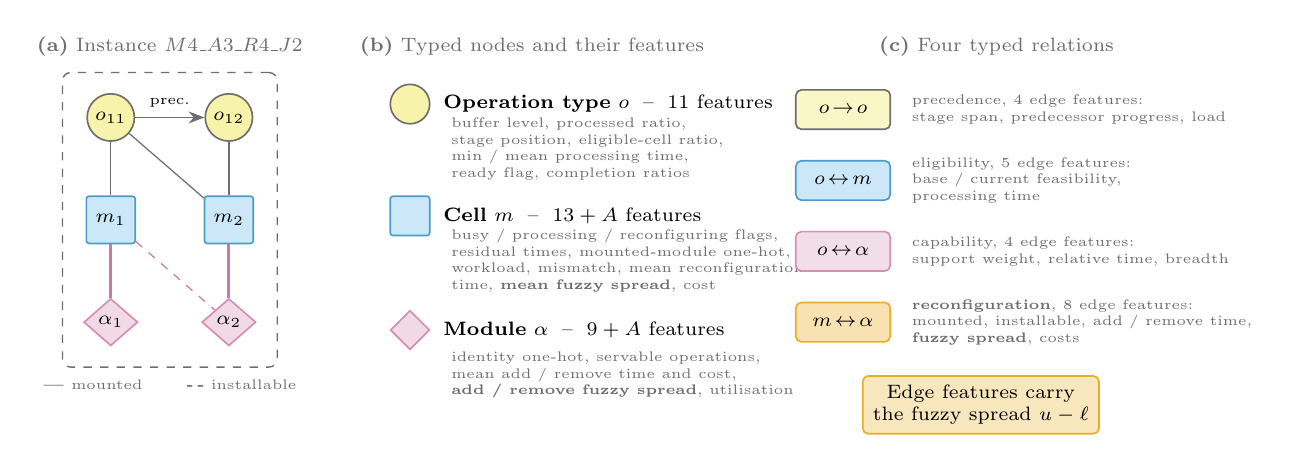
\begin{tikzpicture}

% ---------------- left: a concrete miniature instance ----------------
\node[note] at (0,2.35) {\textbf{(a)} Instance $M4\_A3\_R4\_J2$};

% Three layers, each edge joining adjacent layers only, so no edge passes
% through a node. One job type with two operations is enough to exhibit all
% four relations.
\node[opnode] (o11) at (-0.75,1.45) {$o_{11}$};
\node[opnode] (o12) at ( 0.75,1.45) {$o_{12}$};
\draw[arrow, draw=oigray] (o11) -- node[above, font=\tiny] {prec.} (o12);

\node[macnode] (m1) at (-0.75,0.15) {$m_1$};
\node[macnode] (m2) at ( 0.75,0.15) {$m_2$};
\node[modnode] (a1) at (-0.75,-1.15) {$\alpha_1$};
\node[modnode] (a2) at ( 0.75,-1.15) {$\alpha_2$};

% eligibility: which cell may run which operation
\draw[thinedge] (o11) -- (m1);
\draw[thinedge] (o11) -- (m2);
\draw[thinedge] (o12) -- (m2);
% cell--module: solid and thick where mounted, dashed where installable
\draw[thinedge, draw=oipurple, line width=1.1pt] (m1) -- (a1);
\draw[thinedge, draw=oipurple, dashed] (m1) -- (a2);
\draw[thinedge, draw=oipurple, line width=1.1pt] (m2) -- (a2);

\node[tinynote, align=center] at (0,-1.95)
  {\textbf{---} mounted \qquad \textbf{-\,-} installable};

% ---------------- middle: node types and features --------------------
% Both the headings and the feature lists are set to a narrow measure: at the
% document's own font size a wider one runs straight into panel (c).
\node[note] at (4.6,2.35) {\textbf{(b)} Typed nodes and their features};

\node[opnode, minimum size=5mm] at (3.05,1.62) {};
\node[anchor=west, font=\scriptsize] at (3.35,1.62)
  {\textbf{Operation type} $o$ \;--\; $11$ features};
\node[anchor=west, tinynote, align=left] at (3.45,1.05)
  {buffer level, processed ratio,\\
   stage position, eligible-cell ratio,\\
   min / mean processing time,\\
   ready flag, completion ratios};

\node[macnode, minimum size=5mm] at (3.05,0.20) {};
\node[anchor=west, font=\scriptsize] at (3.35,0.20)
  {\textbf{Cell} $m$ \;--\; $13+A$ features};
\node[anchor=west, tinynote, align=left] at (3.45,-0.37)
  {busy / processing / reconfiguring flags,\\
   residual times, mounted-module one-hot,\\
   workload, mismatch, mean reconfiguration\\
   time, \textbf{mean fuzzy spread}, cost};

\node[modnode, minimum size=5mm] at (3.05,-1.25) {};
\node[anchor=west, font=\scriptsize] at (3.35,-1.25)
  {\textbf{Module} $\alpha$ \;--\; $9+A$ features};
\node[anchor=west, tinynote, align=left] at (3.45,-1.82)
  {identity one-hot, servable operations,\\
   mean add / remove time and cost,\\
   \textbf{add / remove fuzzy spread}, utilisation};

% ---------------- right: relations ------------------------------------
\node[note] at (10.50,2.35) {\textbf{(c)} Four typed relations};

\node[smallblock, fill=oiyellow!30, draw=oigray] (r1) at (8.55,1.55) {$o\!\to\!o$};
\node[smallblock, fill=oisky!30, draw=oiblue!70] (r2) at (8.55,0.65) {$o\!\leftrightarrow\!m$};
\node[smallblock, fill=oipurple!25, draw=oipurple!85] (r3) at (8.55,-0.25) {$o\!\leftrightarrow\!\alpha$};
\node[smallblock, fill=oiorange!30, draw=oiorange!85] (r4) at (8.55,-1.15) {$m\!\leftrightarrow\!\alpha$};

\node[anchor=west, tinynote, align=left] at (9.30,1.55)
  {precedence, $4$ edge features:\\stage span, predecessor progress, load};
\node[anchor=west, tinynote, align=left] at (9.30,0.65)
  {eligibility, $5$ edge features:\\base / current feasibility,\\processing time};
\node[anchor=west, tinynote, align=left] at (9.30,-0.25)
  {capability, $4$ edge features:\\support weight, relative time, breadth};
\node[anchor=west, tinynote, align=left] at (9.30,-1.15)
  {\textbf{reconfiguration}, $8$ edge features:\\
   mounted, installable, add / remove time,\\\textbf{fuzzy spread}, costs};

\node[keyblock, minimum width=30mm, font=\scriptsize, align=center] (out) at (10.30,-2.20)
  {Edge features carry\\the fuzzy spread $u-\ell$};

\begin{scope}[on background layer]
  \node[group, fit=(o11)(o12)(a1)(a2)] {};
\end{scope}
\end{tikzpicture}
\end{document}
